% Options for packages loaded elsewhere
\PassOptionsToPackage{unicode}{hyperref}
\PassOptionsToPackage{hyphens}{url}
\PassOptionsToPackage{dvipsnames,svgnames,x11names}{xcolor}
%
\documentclass[
  letterpaper,
  DIV=11,
  numbers=noendperiod]{scrartcl}

\usepackage{amsmath,amssymb}
\usepackage{iftex}
\ifPDFTeX
  \usepackage[T1]{fontenc}
  \usepackage[utf8]{inputenc}
  \usepackage{textcomp} % provide euro and other symbols
\else % if luatex or xetex
  \usepackage{unicode-math}
  \defaultfontfeatures{Scale=MatchLowercase}
  \defaultfontfeatures[\rmfamily]{Ligatures=TeX,Scale=1}
\fi
\usepackage{lmodern}
\ifPDFTeX\else  
    % xetex/luatex font selection
\fi
% Use upquote if available, for straight quotes in verbatim environments
\IfFileExists{upquote.sty}{\usepackage{upquote}}{}
\IfFileExists{microtype.sty}{% use microtype if available
  \usepackage[]{microtype}
  \UseMicrotypeSet[protrusion]{basicmath} % disable protrusion for tt fonts
}{}
\makeatletter
\@ifundefined{KOMAClassName}{% if non-KOMA class
  \IfFileExists{parskip.sty}{%
    \usepackage{parskip}
  }{% else
    \setlength{\parindent}{0pt}
    \setlength{\parskip}{6pt plus 2pt minus 1pt}}
}{% if KOMA class
  \KOMAoptions{parskip=half}}
\makeatother
\usepackage{xcolor}
\usepackage{soul}
\setlength{\emergencystretch}{3em} % prevent overfull lines
\setcounter{secnumdepth}{-\maxdimen} % remove section numbering
% Make \paragraph and \subparagraph free-standing
\ifx\paragraph\undefined\else
  \let\oldparagraph\paragraph
  \renewcommand{\paragraph}[1]{\oldparagraph{#1}\mbox{}}
\fi
\ifx\subparagraph\undefined\else
  \let\oldsubparagraph\subparagraph
  \renewcommand{\subparagraph}[1]{\oldsubparagraph{#1}\mbox{}}
\fi

\usepackage{color}
\usepackage{fancyvrb}
\newcommand{\VerbBar}{|}
\newcommand{\VERB}{\Verb[commandchars=\\\{\}]}
\DefineVerbatimEnvironment{Highlighting}{Verbatim}{commandchars=\\\{\}}
% Add ',fontsize=\small' for more characters per line
\usepackage{framed}
\definecolor{shadecolor}{RGB}{241,243,245}
\newenvironment{Shaded}{\begin{snugshade}}{\end{snugshade}}
\newcommand{\AlertTok}[1]{\textcolor[rgb]{0.68,0.00,0.00}{#1}}
\newcommand{\AnnotationTok}[1]{\textcolor[rgb]{0.37,0.37,0.37}{#1}}
\newcommand{\AttributeTok}[1]{\textcolor[rgb]{0.40,0.45,0.13}{#1}}
\newcommand{\BaseNTok}[1]{\textcolor[rgb]{0.68,0.00,0.00}{#1}}
\newcommand{\BuiltInTok}[1]{\textcolor[rgb]{0.00,0.23,0.31}{#1}}
\newcommand{\CharTok}[1]{\textcolor[rgb]{0.13,0.47,0.30}{#1}}
\newcommand{\CommentTok}[1]{\textcolor[rgb]{0.37,0.37,0.37}{#1}}
\newcommand{\CommentVarTok}[1]{\textcolor[rgb]{0.37,0.37,0.37}{\textit{#1}}}
\newcommand{\ConstantTok}[1]{\textcolor[rgb]{0.56,0.35,0.01}{#1}}
\newcommand{\ControlFlowTok}[1]{\textcolor[rgb]{0.00,0.23,0.31}{#1}}
\newcommand{\DataTypeTok}[1]{\textcolor[rgb]{0.68,0.00,0.00}{#1}}
\newcommand{\DecValTok}[1]{\textcolor[rgb]{0.68,0.00,0.00}{#1}}
\newcommand{\DocumentationTok}[1]{\textcolor[rgb]{0.37,0.37,0.37}{\textit{#1}}}
\newcommand{\ErrorTok}[1]{\textcolor[rgb]{0.68,0.00,0.00}{#1}}
\newcommand{\ExtensionTok}[1]{\textcolor[rgb]{0.00,0.23,0.31}{#1}}
\newcommand{\FloatTok}[1]{\textcolor[rgb]{0.68,0.00,0.00}{#1}}
\newcommand{\FunctionTok}[1]{\textcolor[rgb]{0.28,0.35,0.67}{#1}}
\newcommand{\ImportTok}[1]{\textcolor[rgb]{0.00,0.46,0.62}{#1}}
\newcommand{\InformationTok}[1]{\textcolor[rgb]{0.37,0.37,0.37}{#1}}
\newcommand{\KeywordTok}[1]{\textcolor[rgb]{0.00,0.23,0.31}{#1}}
\newcommand{\NormalTok}[1]{\textcolor[rgb]{0.00,0.23,0.31}{#1}}
\newcommand{\OperatorTok}[1]{\textcolor[rgb]{0.37,0.37,0.37}{#1}}
\newcommand{\OtherTok}[1]{\textcolor[rgb]{0.00,0.23,0.31}{#1}}
\newcommand{\PreprocessorTok}[1]{\textcolor[rgb]{0.68,0.00,0.00}{#1}}
\newcommand{\RegionMarkerTok}[1]{\textcolor[rgb]{0.00,0.23,0.31}{#1}}
\newcommand{\SpecialCharTok}[1]{\textcolor[rgb]{0.37,0.37,0.37}{#1}}
\newcommand{\SpecialStringTok}[1]{\textcolor[rgb]{0.13,0.47,0.30}{#1}}
\newcommand{\StringTok}[1]{\textcolor[rgb]{0.13,0.47,0.30}{#1}}
\newcommand{\VariableTok}[1]{\textcolor[rgb]{0.07,0.07,0.07}{#1}}
\newcommand{\VerbatimStringTok}[1]{\textcolor[rgb]{0.13,0.47,0.30}{#1}}
\newcommand{\WarningTok}[1]{\textcolor[rgb]{0.37,0.37,0.37}{\textit{#1}}}

\providecommand{\tightlist}{%
  \setlength{\itemsep}{0pt}\setlength{\parskip}{0pt}}\usepackage{longtable,booktabs,array}
\usepackage{calc} % for calculating minipage widths
% Correct order of tables after \paragraph or \subparagraph
\usepackage{etoolbox}
\makeatletter
\patchcmd\longtable{\par}{\if@noskipsec\mbox{}\fi\par}{}{}
\makeatother
% Allow footnotes in longtable head/foot
\IfFileExists{footnotehyper.sty}{\usepackage{footnotehyper}}{\usepackage{footnote}}
\makesavenoteenv{longtable}
\usepackage{graphicx}
\makeatletter
\def\maxwidth{\ifdim\Gin@nat@width>\linewidth\linewidth\else\Gin@nat@width\fi}
\def\maxheight{\ifdim\Gin@nat@height>\textheight\textheight\else\Gin@nat@height\fi}
\makeatother
% Scale images if necessary, so that they will not overflow the page
% margins by default, and it is still possible to overwrite the defaults
% using explicit options in \includegraphics[width, height, ...]{}
\setkeys{Gin}{width=\maxwidth,height=\maxheight,keepaspectratio}
% Set default figure placement to htbp
\makeatletter
\def\fps@figure{htbp}
\makeatother

\usepackage{booktabs}
\usepackage{longtable}
\usepackage{array}
\usepackage{multirow}
\usepackage{wrapfig}
\usepackage{float}
\usepackage{colortbl}
\usepackage{pdflscape}
\usepackage{tabu}
\usepackage{threeparttable}
\usepackage{threeparttablex}
\usepackage[normalem]{ulem}
\usepackage{makecell}
\usepackage{xcolor}
\usepackage{siunitx}

  \newcolumntype{d}{S[
    input-open-uncertainty=,
    input-close-uncertainty=,
    parse-numbers = false,
    table-align-text-pre=false,
    table-align-text-post=false
  ]}
  
\KOMAoption{captions}{tableheading}
\makeatletter
\makeatother
\makeatletter
\makeatother
\makeatletter
\@ifpackageloaded{caption}{}{\usepackage{caption}}
\AtBeginDocument{%
\ifdefined\contentsname
  \renewcommand*\contentsname{Table of contents}
\else
  \newcommand\contentsname{Table of contents}
\fi
\ifdefined\listfigurename
  \renewcommand*\listfigurename{List of Figures}
\else
  \newcommand\listfigurename{List of Figures}
\fi
\ifdefined\listtablename
  \renewcommand*\listtablename{List of Tables}
\else
  \newcommand\listtablename{List of Tables}
\fi
\ifdefined\figurename
  \renewcommand*\figurename{Figure}
\else
  \newcommand\figurename{Figure}
\fi
\ifdefined\tablename
  \renewcommand*\tablename{Table}
\else
  \newcommand\tablename{Table}
\fi
}
\@ifpackageloaded{float}{}{\usepackage{float}}
\floatstyle{ruled}
\@ifundefined{c@chapter}{\newfloat{codelisting}{h}{lop}}{\newfloat{codelisting}{h}{lop}[chapter]}
\floatname{codelisting}{Listing}
\newcommand*\listoflistings{\listof{codelisting}{List of Listings}}
\makeatother
\makeatletter
\@ifpackageloaded{caption}{}{\usepackage{caption}}
\@ifpackageloaded{subcaption}{}{\usepackage{subcaption}}
\makeatother
\makeatletter
\@ifpackageloaded{tcolorbox}{}{\usepackage[skins,breakable]{tcolorbox}}
\makeatother
\makeatletter
\@ifundefined{shadecolor}{\definecolor{shadecolor}{rgb}{.97, .97, .97}}
\makeatother
\makeatletter
\makeatother
\makeatletter
\makeatother
\ifLuaTeX
  \usepackage{selnolig}  % disable illegal ligatures
\fi
\IfFileExists{bookmark.sty}{\usepackage{bookmark}}{\usepackage{hyperref}}
\IfFileExists{xurl.sty}{\usepackage{xurl}}{} % add URL line breaks if available
\urlstyle{same} % disable monospaced font for URLs
\hypersetup{
  pdftitle={Cooperative Recreational Sampling Program},
  colorlinks=true,
  linkcolor={blue},
  filecolor={Maroon},
  citecolor={Blue},
  urlcolor={Blue},
  pdfcreator={LaTeX via pandoc}}

\title{Cooperative Recreational Sampling Program}
\usepackage{etoolbox}
\makeatletter
\providecommand{\subtitle}[1]{% add subtitle to \maketitle
  \apptocmd{\@title}{\par {\large #1 \par}}{}{}
}
\makeatother
\subtitle{Standard Operating Procedures}
\author{}
\date{}

\begin{document}
\maketitle
\ifdefined\Shaded\renewenvironment{Shaded}{\begin{tcolorbox}[sharp corners, breakable, enhanced, frame hidden, interior hidden, borderline west={3pt}{0pt}{shadecolor}, boxrule=0pt]}{\end{tcolorbox}}\fi

\hypertarget{contact-information}{%
\subsection{Contact Information}\label{contact-information}}

\textbf{Melissa Monk}, \emph{NOAA Southwest Fisheries Science Center
(SWFSC)}, \textbf{email:} \url{melissa.monk@noaa.gov}

\textbf{Kenneth Franke}, \emph{Sportfishing Association of California
(SAC),} \textbf{email:} \url{kennethfrankesac@gmail.com}

\textbf{Rachel Brooks}, \emph{NOAA Southwest Fisheries Science Center
(SWFSC)}, \textbf{email:} \url{rachel.brooks@noaa.gov}

\textbf{Merit McCrea}, \emph{Sportfishing Association of California
(SAC),} \textbf{email:}
\href{edwin@sportfishca.org}{meritmmcrea@hotmail.com}

\textbf{Edwin Reyes}, \emph{Sportfishing Association of California
(SAC),} \textbf{email:} \url{edwin@sportfishca.org}

\hypertarget{background}{%
\subsection{Background}\label{background}}

The 2018 Marine Life Management Act Master Plan for fisheries
specifically recommends prioritizing additional environmental and
fisheries monitoring to increase climate resiliency. Biological sampling
of targeted fishes is critical to understanding the effects of
environmental change and the corresponding impacts on managed fisheries,
and can provide the baseline data needed to manage a fishery for
increased ecological resilience. In addition to increasing
climate-resiliency, monitoring and sampling life-history characteristics
of targeted species is necessary for adaptive management, where knowing
how specific age/size classes within a fishery are being impacted is the
first step in developing management strategies that guard against
over-exploitation.~

While CDFW currently surveys the landings and length distributions of
rockfishes encountered by the recreational fishing fleet as part of the
California Recreational Fisheries Survey (CRFS); CRFS does not currently
collect otoliths (for age and growth), fin clips (for genetic analyses),
or any other biological information only available from examining the
internal organs of a fish (i.e., sex, maturity status, fecundity,
condition). This lack of sampling means that many management decisions
are currently being made with incomplete or insufficient data, leading
to uncertainty in the assessments and questioning of the
process/outcomes by stakeholders.~

Additionally, the lack of sampling leads to a critical lack of
information about the spatial scale of how targeted species are reacting
to both fishing pressure and climate change. Specifically, how life
history traits are changing in response to marine heatwaves and other
local climate change effects. This is particularly important for
reef-associated nearshore fishes, as they occupy habitats likely to be
impacted most by changing ocean conditions.

In partnership with the Sportfishing Association of California (SAC),
the NOAA Fisheries Ecology Division (FED) at the Southwest Fisheries
Science Center is piloting a \# year-long cooperative sampling project
to collect biological samples for groundfishes from the for-hire
recreational fishing fleet across California. Vessel captains and crew
members are trained to measure and retain groundfish samples of specific
target species (see Vessel Sampling Protocols for more details). The
samples are then labeled, organized, preserved and shipped to NOAA SWFSC
and California Collaborative Fisheries Research Program (CCFRP) campuses
for further dissections and analysis. The life history information
generated from this biological data are incorporated into current
federal stock assessment efforts.

\hypertarget{project-objectives}{%
\subsubsection{Project Objectives:}\label{project-objectives}}

\begin{enumerate}
\def\labelenumi{\arabic{enumi}.}
\item
  Collect information on federally-managed groundfish species in
  cooperation with the Sportfishing Association of California (SAC) and
  the California commercial passenger fishing vessel (CPFV) fleet during
  the recreational fishing season to inform stock assessments and
  management.
\item
  Charter CPFVs during months when rockfish are spawning for additional
  biological data on maturity and fecundity.
\end{enumerate}

\hypertarget{cdfw-recreational-groundfish-season-structure}{%
\subsection{2023 CDFW Recreational Groundfish Season
Structure}\label{cdfw-recreational-groundfish-season-structure}}

\begin{Shaded}
\begin{Highlighting}[]
\CommentTok{\#| label: fig{-}include{-}figure}
\CommentTok{\#| out{-}width: "900px"}
\CommentTok{\#| fig{-}cap: "2023 recreational groundfish season structure separated by CDFW management areas"}
\CommentTok{\#| fig{-}alt: "2023 recreational groundfish season structure separated by CDFW management areas"}
\NormalTok{knitr}\SpecialCharTok{::}\FunctionTok{include\_graphics}\NormalTok{(}\StringTok{"CDFW{-}regulation.PNG"}\NormalTok{)}
\end{Highlighting}
\end{Shaded}

\begin{figure}[H]

{\centering \includegraphics{CDFW-regulation.PNG}

}

\end{figure}

\hypertarget{in-season-groundfish-regulation-changes}{%
\subsubsection{2023 In-Season Groundfish Regulation
Changes:}\label{in-season-groundfish-regulation-changes}}

\begin{itemize}
\item
  \textbf{Effective August 7th, 2023:} Retention of quillback rockfish
  (\emph{Sebastes maliger}) is prohibited statewide in both the
  recreational and commercial fisheries - \emph{announced July 28th,
  2023}
\item
  \textbf{Effective August 21st, 2023:} Recreational boat-based
  groundfish fishing will only be permitted seaward of the 50 fathom
  Rockfish Conservation Area (RCA) boundary line for the Northern
  Groundfish Management Area (GMA) - \emph{announced August 11th, 2023}
\item
  \textbf{Effective September 1st, 2023:} Recreational boat-based
  groundfish fishing will only be permitted seaward of the 50 fathom
  Rockfish Conservation Area (RCA) boundary line for the Mendocino
  Groundfish Management Area (GMA), San Francisco GMA, and Central Coast
  GMA - \emph{announced August 21st, 2023}
\end{itemize}

\hypertarget{vessel-sampling-protocols}{%
\subsection{Vessel Sampling Protocols}\label{vessel-sampling-protocols}}

To collect life history information on groundfish species in cooperation
with the California CPFV fleet, we have identified several different
potential methods that we will explore during the 2023 fishing season.~
These three methods are all preliminary and the program will adapt based
on feedback from the fleet and scientists. Each vessel/landing will
receive training and instructions specific to their protocol.

\hypertarget{on-board-sampling-by-vessel-crew-members}{%
\subsubsection{On-Board Sampling by Vessel Crew
Members}\label{on-board-sampling-by-vessel-crew-members}}

Every 1-2 month period, or as needed, each vessel will receive 50 tags.
The expectation is to sample 50 fish over the course of one month, and,
to the extent possible, distribute the sampling evenly over the 1-month
period.

Each sampled fish will be tagged through the lower jaw/operculum with a
Tyvek tag that is pre-labelled with the vessel name and species, and
will be measured on a provided~ L-shaped measuring board by a crew
member prior to fileting. The crew will measure the fish and record the
length and capture date with permanent ink (a ``sharpie'') on the Tyvek
tag. Once the fish has been measured, the crew can filet the fish
leaving the stomach cavity intact for later sex and maturity stage
determination. The tagged carcass will then be placed in a contractor
trash bag and cooler and stored in a freezer prior to being shipped or
picked up by NMFS or CCFRP researchers for laboratory processing.

Each vessel will be compensated \$300 a month for participation in this
cooperative sampling contingent on providing 50 samples per month.

\href{https://drive.google.com/file/d/1OFiml_G4lwsWu2RsiYxac2mk8eRYo7p9/view?usp=sharing}{\textbf{6-PAX
Vessels:}} 25 tags per species for a predetermined suite of groundfish
(e.g., rockfish, greenlings, California scorpionfish), along with tags
for opportunistic sampling of less commonly encountered species (i.e.,
BONUS tags) will be provided. The flexibility of having tags for
multiple species is needed to ensure collection of adequate sample sizes
for assessments. One motivation for providing tags for a suite of
species is that vessels fishing in an area where ``All Depths'' are open
may fish farther from port on good weather days and closer to port
during sub-optimal conditions, resulting in different species
compositions in the catch.

The vessel crew will sample no more than 25 fish per trip. On a given
trip, the vessel crew will sample all tagged species kept by anglers on
trips until they have reached 25 of each. The vessel crew can fill in
with BONUS samples as needed with a maximum of 8 fish per trip.

\href{https://drive.google.com/file/d/10tcgyl3dkq_NRH5TrU9DeakOrtZvPEXL/view?usp=sharing}{\textbf{Party
Boat Vessels Option A (sample up to 50 fish per trip):}} 25 tags per
species for a predetermined suite of groundfish (e.g., rockfish,
greenlings, California scorpionfish), along with tags for opportunistic
sampling of less commonly encountered species (i.e., BONUS tags) will be
provided. The flexibility of having tags for multiple species is needed
to ensure collection of adequate sample sizes for assessments. One
motivation for providing tags for a suite of species is that vessels
fishing in an area where ``All Depths'' are open may fish farther from
port on good weather days and closer to port during sub-optimal
conditions, resulting in different species compositions in the catch.

The vessel crew will sample no more than 50 fish from a single trip per
month, and may sample multiple trips if needed to reach 50 fish for the
month. On a given trip, the vessel crew will pick two species to sample
from the species tags. For one species, the vessel crew will sample 1-2
fish from all odd numbered angler bags (1,3,5, etc.) until they reach
25. The vessel crew will sample 1-2 fish of the second species from all
even numbered angler bags (2,4,6, etc.) until they reach 25. The 1-2
fish of the same species will be selected randomly from the bag.

\href{https://drive.google.com/file/d/14bi-9TEZSylgiLCytEaThr1CO-3Eljon/view?usp=sharing}{\textbf{Party
Boat Vessels Option B (sample up to 25 fish per trip):}} 25 tags per
species for a predetermined suite of groundfish (e.g., rockfish,
greenlings, California scorpionfish), along with tags for opportunistic
sampling of less commonly encountered species (i.e., BONUS tags) will be
provided. The flexibility of having tags for multiple species is needed
to ensure collection of adequate sample sizes for assessments. One
motivation for providing tags for a suite of species is that vessels
fishing in an area where ``All Depths'' are open may fish farther from
port on good weather days and closer to port during sub-optimal
conditions, resulting in different species compositions in the catch.

The vessel crew will sample at least 25 fish on two trips per month. On
the first trip, the vessel crew will pick one of the two species to
sample from the assigned species tags. The vessel crew will randomly
sample 1-2 individuals from all odd numbered angler bags (1,3,5, etc.)
until they reach 25. On the second trip, the crew will follow the same
procedure for the second species.

\href{https://drive.google.com/file/d/1rIka7pY_DXWL-FqTUodazEqWex9ovj0W/view?usp=sharing}{\textbf{Party
Boat Vessels Option C (sample whole bags):}} 50 write-in species tags
will be provided each month. The vessel crew will identify 3-5 volunteer
anglers to have their bags sampled prior to having their fish filleted.
The vessel crew will sample a subset of species using the following
procedures: (1) the sampler will measure and tag two randomly selected
vermilion rockfish from each bag; (2) the sampler will measure and tag
all other species in the bag except bank rockfish, chilipepper rockfish,
widow rockfish, and bocaccio rockfish. Although this tag provides an
extra step of writing in the species, it will provide greater
flexibility and opportunity to sample throughout the groundfish season.

\hypertarget{on-board-sampling-by-nmfsccfrp-researcher}{%
\subsubsection{On-Board Sampling by NMFS/CCFRP
Researcher}\label{on-board-sampling-by-nmfsccfrp-researcher}}

\href{https://drive.google.com/file/d/1o7kY7kULP_budD7yP4ZCjEFSpdjwJd3N/view?usp=sharing}{\textbf{On-Board
Sampling by Researcher:}} One to three times per month, a NMFS or CCFRP
researcher will coordinate with the vessel to ride along on a fishing
charter to sample the catch from the trip. The sampler will identify 5-7
anglers to have their bags sampled prior to having their fish filleted.
The NMFS or CCFRP sampler will sample a subset of species using the
following procedures: (1) the sampler will measure and tag two randomly
selected vermilion rockfish from each bag; (2) the sampler will measure
and tag all other species in the bag except bank rockfish, chilipepper
rockfish, widow rockfish, and bocaccio rockfish. In addition to the 5
bags, the sampler will opportunistically measure and tag priority
species (i.e., copper rockfish, quillback rockfish) or less commonly
encountered species (e.g., tiger rockfish, flag rockfish) onboard.~

Each sampled fish will be tagged through the lower jaw/operculum with a
Tyvek tag that is pre-labelled with the vessel name and species, and
will be measured on an L-shaped measuring board by the NMFS or CCFRP
sampler.~ The tag will indicate to the crew that the fish was selected
for sampling. The NMFS or CCFRP sampler will measure the fish and record
the length and capture date with a sharpie on the Tyvek tag. Once the
fish has been measured by the NMFS or CCFRP sampler, the crew can filet
the fish leaving the stomach cavity intact for later sex and maturity
stage determination. The carcass will be handed off to the NMFS or CCFRP
sampler for immediate processing either at the dock or back at the
laboratory facility.~~

This sampling may occur in tandem with an onboard observer trip
conducted by Cal Poly SLO, and in other locations, if the captains
agree, similar onboard observer data will be collected during a
ride-along.~ All information that the vessel considers proprietary or
confidential will remain confidential. Each vessel will be compensated
\$300 each month for participation in this cooperative sampling.

\hypertarget{dockside-sampling-by-nmfsccfrp-researcher}{%
\subsubsection{Dockside Sampling by NMFS/CCFRP
Researcher}\label{dockside-sampling-by-nmfsccfrp-researcher}}

\href{https://drive.google.com/file/d/19i_ubpa1QG1Ra2br7qk-RAFmMVGjmr5J/view?usp=sharing}{\textbf{On-Dock
Sampling by Researcher:}} One to three times a month, a NMFS or CCFRP
researcher will coordinate with the vessel operator to sample the catch
from the trip once the vessel returns to the fishing dock. At the start
of the trip the vessel crew will identify 5 customers willing to have
their bags sampled back at the dock prior to having their fish fileted.~
The NMFS or CCFRP sampler will meet the vessel at the dock and sample a
subset of species using the following procedures: (1) the sampler will
sample only two randomly selected vermilion rockfish from each bag; (2)
the sampler will sample all other species in the bag except bank
rockfish, chilipepper rockfish, widow rockfish and bocaccio rockfish.~

Each sampled fish will be tagged through the lower jaw/operculum with a
Tyvek tag that is pre-labelled with the vessel name and species, and
will be measured on an L-shaped measuring board by the NMFS or CCFRP
sampler prior to filleting. To measure the fish, the NMFS or CCFRP
sampler will position the fish flat on the measuring board with the
mouth closed and pressed up against the tip of the board at the zero
line with the caudal fin splayed out and not pinched. The NMFS or CCFRP
sampler will measure the fish to the nearest millimeter at the center of
the caudal fin and record the length and capture date with a sharpie on
the Tyvek tag. Once the fish has been measured by the NMFS or CCFRP
sampler, the crew can filet the fish leaving the stomach cavity intact
for later sex and maturity stage determination. The carcass will be
handed off to the NMFS or CCFRP sampler for processing either at the
dock or back at the laboratory facility.

Each vessel will be compensated \$300 each month for participation in
this cooperative sampling.

\begin{Shaded}
\begin{Highlighting}[]
\CommentTok{\#| label: fig{-}include{-}figure}
\CommentTok{\#| out{-}width: "400px"}
\CommentTok{\#| fig{-}cap: "Example of a tagged and filleted Copper Rockfish (Sebastes carnatus) sample"}
\CommentTok{\#| fig{-}alt: "Example of a tagged and filleted Copper Rockfish (Sebastes carnatus) sample"}
\NormalTok{knitr}\SpecialCharTok{::}\FunctionTok{include\_graphics}\NormalTok{(}\StringTok{"Copper{-}Rockfish{-}Sample.png"}\NormalTok{)}
\end{Highlighting}
\end{Shaded}

\begin{figure}[H]

{\centering 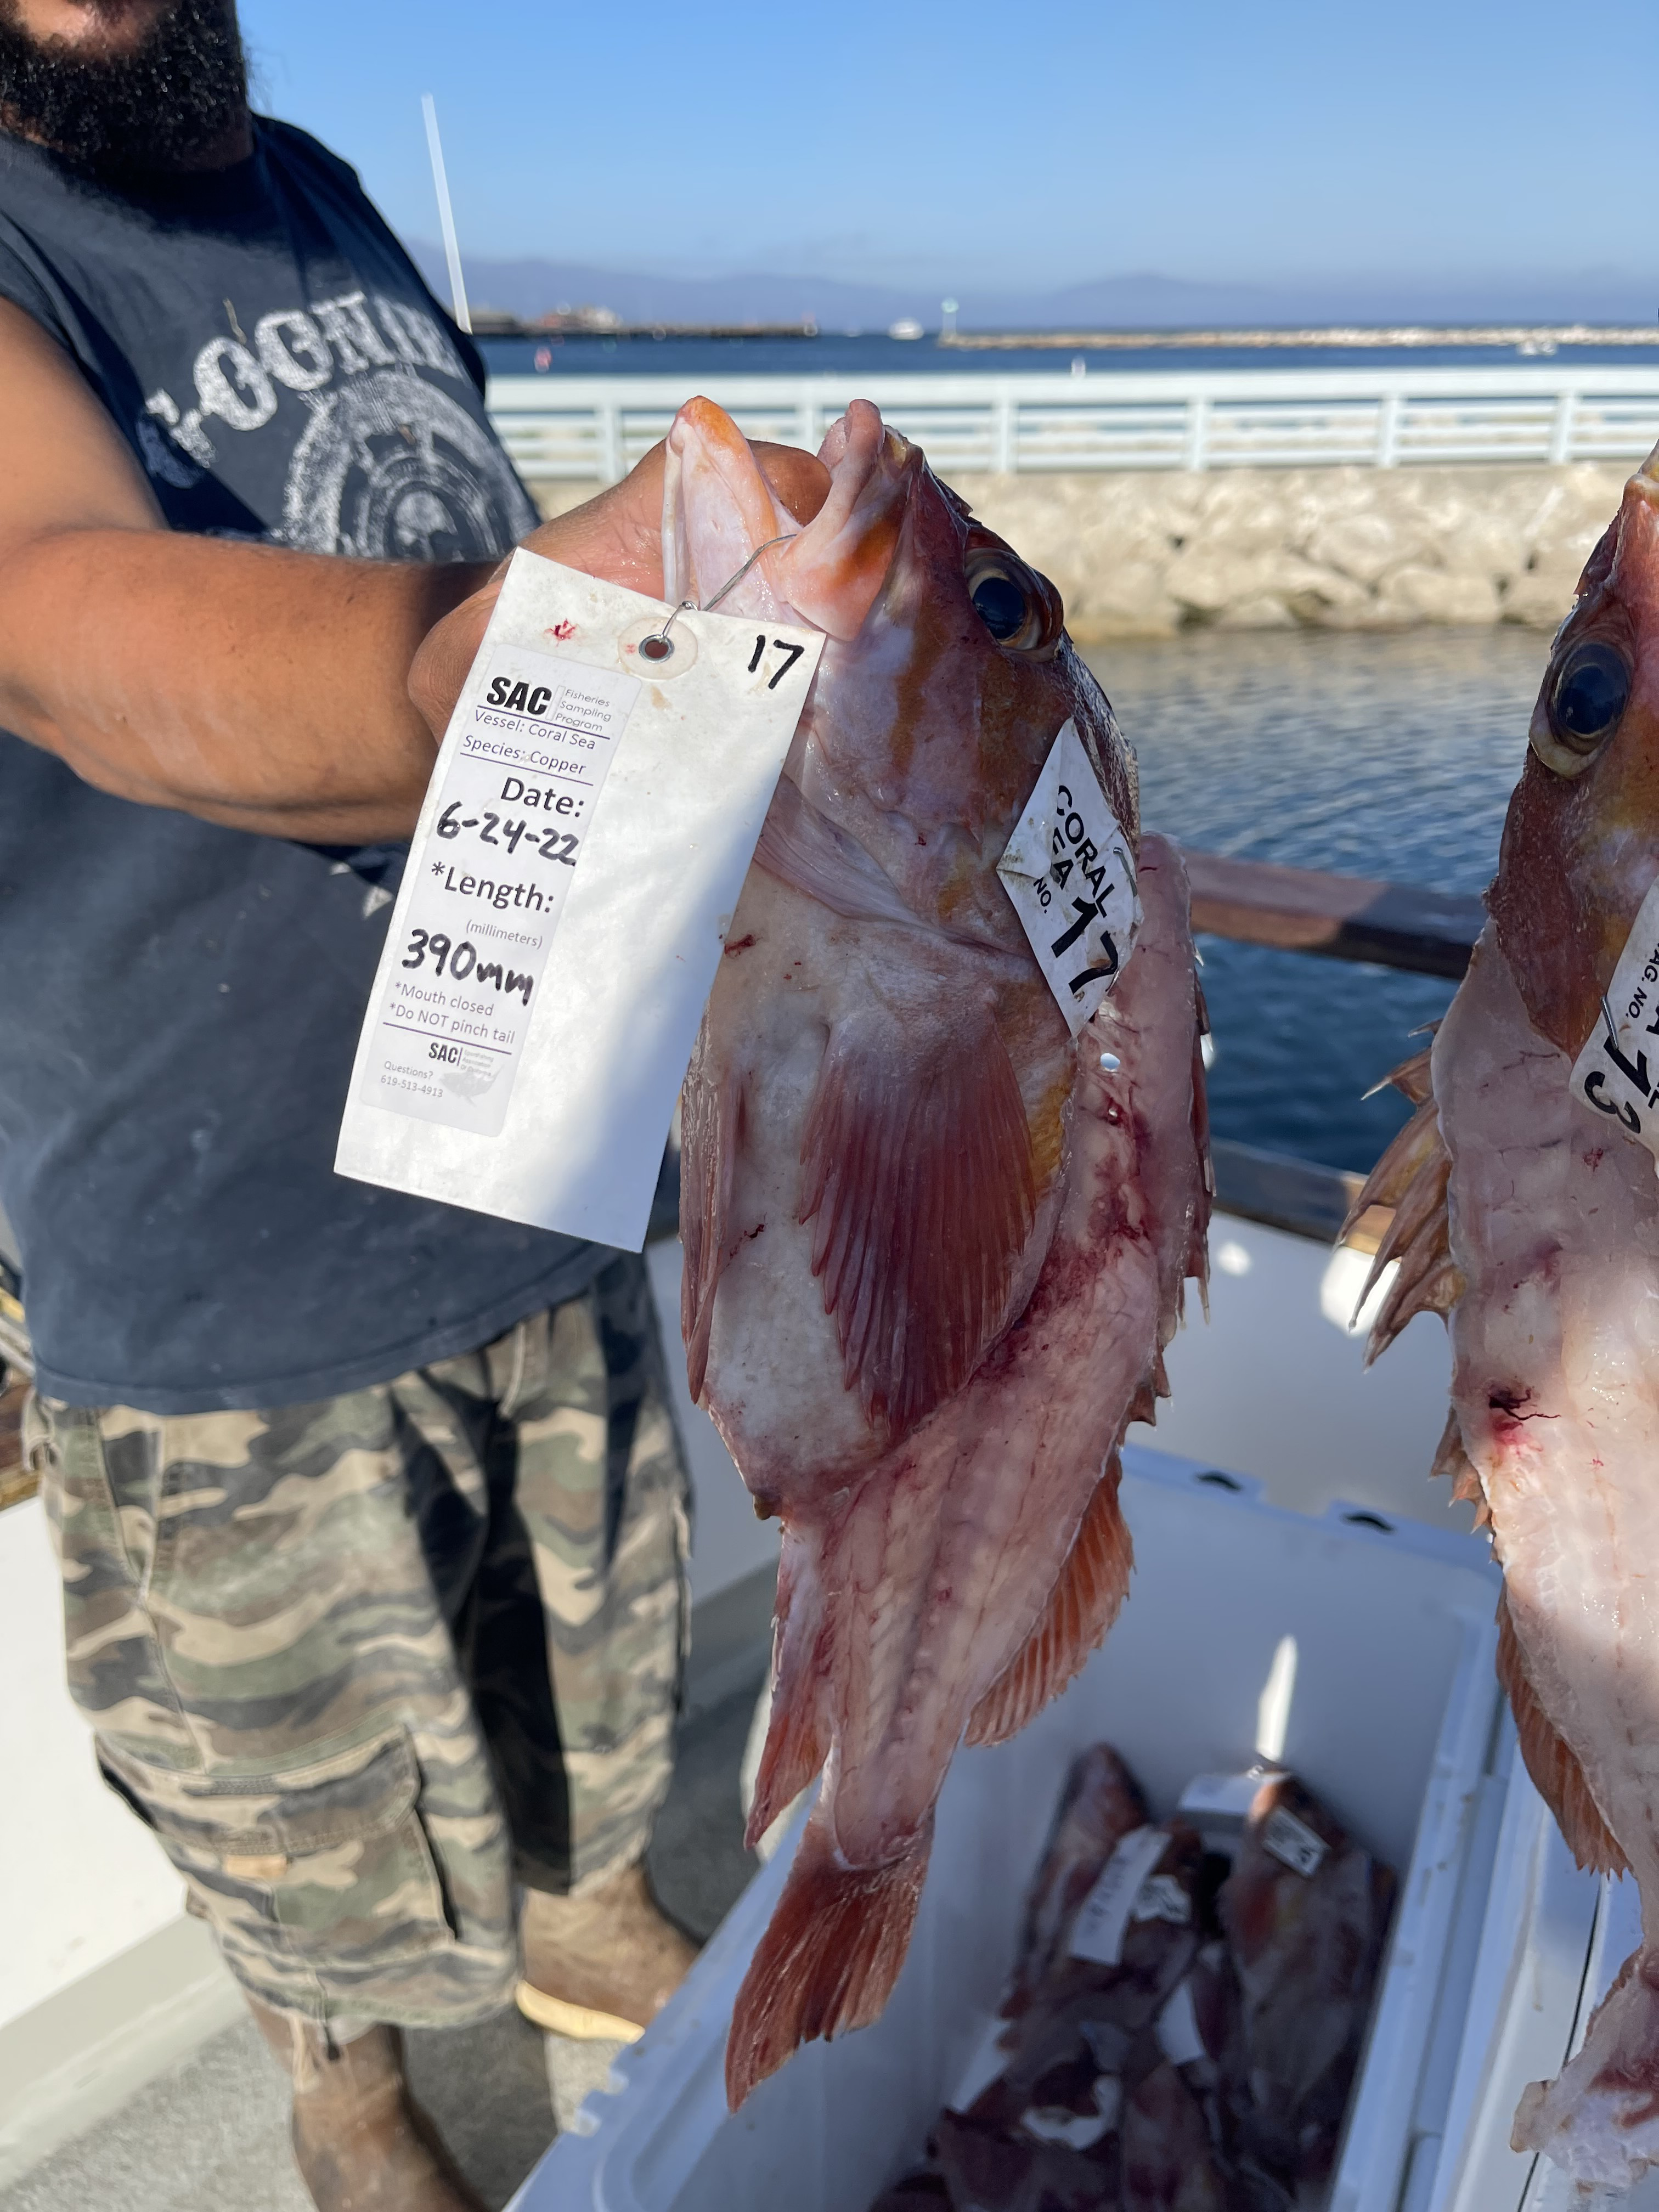
\includegraphics{Copper-Rockfish-Sample.png}

}

\end{figure}

\hypertarget{participating-vessels}{%
\subsection{Participating Vessels}\label{participating-vessels}}

Vessels participating in the 2023 Cooperative Recreational Sampling
Program (CRSP)

\begin{longtable}[]{@{}
  >{\centering\arraybackslash}p{(\columnwidth - 10\tabcolsep) * \real{0.3151}}
  >{\centering\arraybackslash}p{(\columnwidth - 10\tabcolsep) * \real{0.1370}}
  >{\centering\arraybackslash}p{(\columnwidth - 10\tabcolsep) * \real{0.1370}}
  >{\centering\arraybackslash}p{(\columnwidth - 10\tabcolsep) * \real{0.1370}}
  >{\centering\arraybackslash}p{(\columnwidth - 10\tabcolsep) * \real{0.1370}}
  >{\centering\arraybackslash}p{(\columnwidth - 10\tabcolsep) * \real{0.1370}}@{}}
\toprule\noalign{}
\begin{minipage}[b]{\linewidth}\centering
Vessel Name
\end{minipage} & \begin{minipage}[b]{\linewidth}\centering
Port
\end{minipage} & \begin{minipage}[b]{\linewidth}\centering
CDFW Boat \#
\end{minipage} & \begin{minipage}[b]{\linewidth}\centering
CDFW Management Region
\end{minipage} & \begin{minipage}[b]{\linewidth}\centering
Vessel Type
\end{minipage} & \begin{minipage}[b]{\linewidth}\centering
CRSP Vessel Sampling Protocol
\end{minipage} \\
\midrule\noalign{}
\endhead
\bottomrule\noalign{}
\endlastfoot
\href{https://www.hmlanding.com/boat/premier}{\emph{Premier}} & San
Diego & 03233 & Southern & Party Boat & Vessel On-Board Sampling (C) \\
\href{https://danawharf.com/our-boats/sum-fun/}{\emph{Sum Fun}} & Dana
Wharf & 12360 & Southern & Party Boat & Vessel On-Board Sampling (C) \\
\href{https://www.eldoradosportfishing.com/}{\emph{Eldorado}} & Long
Beach & 16699 & Southern & Party Boat & Vessel On-Board Sampling (C) \\
\href{https://mdrsf.com/betty-o/}{\emph{Betty-O}} & Marina Del Rey &
04990 & Southern & Party Boat & Vessel On-Board Sampling (B) \\
\href{https://www.miragesportfishing.com/}{\emph{Mirage}} & Channel
Islands & 28054 & Southern & Party Boat & Vessel On-Board Sampling
(B) \\
\href{https://www.stardustsportfishing.com/galleries/1058-stardust-gallery}{\emph{Stardust}}
& Santa Barbara & 39022 & Southern & Party Boat & Vessel On-Board
Sampling (B) \\
\href{https://www.stardustsportfishing.com/galleries/1056-the-coral-sea}{\emph{Coral
Sea}} & Santa Barbara & 12758 & Southern & Party Boat & Vessel On-Board
Sampling (B) \\
\href{https://patriotsportfishing.com/patriot/}{\emph{Patriot}} & Avila
Beach & 02214 & Central & Party Boat & Dockside Sampling CCFRP \\
\href{virgslanding.com/fleet-safety/fiesta-3/}{\emph{Fiesta}} & Morro
Bay & 33680 & Central & Party Boat & Dockside Sampling CCFRP \\
\href{https://www.lastmealsportfishing.com/}{\emph{Last Meal}} & Moss
Landing & 73873 & Central & 6-PAX & Dockside Sampling CCFRP \\
\href{https://www.kahunasportfishing.com/}{\emph{Kahuna}} & Moss Landing
& 38325 & Central & Party Boat & Vessel On-Board Sampling (C) \\
\href{https://www.klughersportfishing.com/}{\emph{Queen of Hearts}} &
Half Moon Bay & 37423 & San Francisco & Party Boat & Vessel On-Board
Sampling (B) \\
\href{https://www.seawolfsportfishing.com/}{\emph{Sea Wolf}} &
Emeryville & 29746 & San Francisco & Party Boat & Vessel On-Board
Sampling (B) \\
\href{https://www.bodegacharters.com/}{\emph{New Sea Angler}} & Bodega
Bay & 30068 & San Francisco & Party Boat & Dockside Sampling CCFRP \\
\href{https://anchorcharterboats.com/the-kraken/}{\emph{Kraken}} & Fort
Bragg & 72865 & Mendocino & Party Boat & Vessel On-Board Sampling (B) \\
\href{https://fishtanksite.com/}{\emph{Kyndall Lynn}} & Fort Bragg &
06810 & Mendocino & 6-PAX & 6-PAX Vessel On-Board Sampling \\
\href{https://seahawksportfishing.com/}{\emph{Sea Hawk}} & Shelter Cove
& 05978 & Mendocino & 6-PAX & 6-PAX Vessel On-Board Sampling \\
\href{http://reelsteelsportfishing.com/}{\emph{New Reel Steel}} & Eureka
& 71226 & Northern & 6-PAX & 6-PAX Vessel On-Board Sampling \\
\href{https://coastlinefishingcharters.com/}{\emph{Scrimshaw}} & Eureka
& 71246 & Northern & 6-PAX & 6-PAX Vessel On-Board Sampling \\
\end{longtable}

\hypertarget{vessel-tags}{%
\subsection{Vessel Tags}\label{vessel-tags}}

\hypertarget{assigning-tracking-vessel-tags}{%
\subsubsection{Assigning \& Tracking Vessel
Tags}\label{assigning-tracking-vessel-tags}}

Vessel tags are provided to each participating vessel on a monthly
basis. Species tags are decided based on current inventory and feedback
from the vessel captain and/or crew. Vessel tags are tracked within the
\href{https://docs.google.com/spreadsheets/d/1hVaB7Wh5BB_hfSLxPLvWwM52cUw4IfROGIHiH_5Y8YM/edit?usp=sharing}{Rockfish
Sampling Contacts and Records} spreadsheet under the respective vessel's
tab. For a given vessel each month, information on the assigned species
and number of tags sent for each species is recorded, as well as the
date in which tags were shipped and who the tags were shipped by.

\hypertarget{making-vessel-tags}{%
\subsubsection{Making Vessel Tags}\label{making-vessel-tags}}

Vessel labels and species labels for tags are created through Avery.
Labels are made for a 1'' x 2 5/8'' Easy peel address label template
\#5136 (produces 30 labels). Most vessel and species labels are
downloaded as a PDF from Avery and stored in the
\href{https://drive.google.com/drive/folders/1RhFYLp9Z7GObnFLIC52e8ql9CKm6dATv?usp=drive_link}{Labels
for Printing Folder} in the Cooperative Recreational Sampling Google
Drive.

\ul{\textbf{Avery Account Information:}}

\textbf{Email:} \emph{swfsc.groundfish@noaa.gov}

\textbf{Password:} \emph{!likeR0ckfish!}

\begin{Shaded}
\begin{Highlighting}[]
\CommentTok{\#| label: fig{-}include{-}figure}
\CommentTok{\#| out{-}width: "400px"}
\CommentTok{\#| fig{-}cap: "Vessel tag example"}
\CommentTok{\#| fig{-}alt: "Vessel tag example"}
\NormalTok{knitr}\SpecialCharTok{::}\FunctionTok{include\_graphics}\NormalTok{(}\StringTok{"Vessel{-}Tag.png"}\NormalTok{)}
\end{Highlighting}
\end{Shaded}

\begin{figure}[H]

{\centering \includegraphics{Vessel-Tag.png}

}

\end{figure}

\hypertarget{shipping-vessel-tags}{%
\subsubsection{Shipping Vessel Tags}\label{shipping-vessel-tags}}

Vessel tags are shipped monthly - either within the last week or first
week of each month. Tags are shipped via the Sportfishing Association of
California's (SAC) USPS Business Account.

\ul{\textbf{SAC USPS Account Information:}}

\textbf{User Name:} \emph{SAC-Deliveries}

\textbf{Password:} \emph{FisheriesProjects2023!}

\begin{enumerate}
\def\labelenumi{\arabic{enumi}.}
\item
  To ship tags, log into USPS account. Under `Quick Tools' select
  `Click-and-Ship'. Scroll down and select `Create a Single Label'.
\item
  For Step 1, key-in relevant delivery address information in (NOTE:
  Most shipping addresses are saved in the SAC accounts Address Book)
  and check `No' for `\emph{Are you shipping dangerous goods or
  hazardous materials}?'
\item
  For Step 2, key-in relevant shipping information. Tags are typically
  sent in non-USPS 10 in x 7 in bubble mailer envelopes and are sent via
  USPS Ground Advantage (starting at \$3.59 per package and delivered
  within 2-5 days).
\item
  Select `Add to Cart' and make additional packing slips (if shipping
  tags to more than one vessel). Once all packing slips are created, go
  to shopping cart and select `Pay Now'.
\item
  At checkout, select `Credit \& Debit Card' and input the 3-digit CVC
  (\emph{323}), then click `Print \& Pay'. This will take you to a new
  page where you can download a PDF copy of the shipping label/receipt.
\item
  Download and print the shipping label and attach to the package.
\item
  To keep track of vessel tag shipping expenses, save a copy of the
  shipping label/receipt to the
  \href{https://drive.google.com/drive/folders/1Au1fgI4Q4YLSMRgdUK6k4wnxC3-nAtSh?usp=drive_link}{USPS
  Receipts Folder}. Additionally, make sure to add in a line item charge
  for each shipping label to the
  `\href{https://docs.google.com/spreadsheets/d/1B21y44leBmms9Unx1HGpoDxx2XMXN5p7k_OTchB_RWg/edit?usp=sharing}{PSMFC
  23-001C; SAC 1247.23' tab of the PSMFC Funds Budget Spreadsheet}.
  Under the 'Item' column, list `Supplies - USPS shipping tags
  \ul{\emph{Insert Month}} \emph{- \ul{Insert Vessel Name or CCFRP
  Institution}';} under the 'Encumbered Funds' column, list the price of
  the individual shipping label (should not exceed \$5.00); under the
  `Notes' column, list the date in which the tags were shipped.
\end{enumerate}

\hypertarget{tracking-vessel-samples}{%
\subsection{Tracking Vessel Samples}\label{tracking-vessel-samples}}

Vessel samples are tracked two-fold via routine monthly check-in's with
participating vessels and via data entry tracking. Data collected from
sampled carcasses are entered into a Google Sheets Database by
participating CCFRP institution. Each institution enters dissection data
within their own tab on Google Sheets , then the data is merged using
the Query function. The dissection data are auto-populated into the
vessel specific tabs within the
\href{https://docs.google.com/spreadsheets/d/1hVaB7Wh5BB_hfSLxPLvWwM52cUw4IfROGIHiH_5Y8YM/edit\#gid=1355710864}{Rockfish
Sampling Contacts and Records} Database. Once a vessel reaches 50
samples, a box is checked manually by Rachel Brooks to signal vessel is
ready for payment and triggers notification to Merit McCrea to process
payment. All subsequent tables are up to date data from the Google
Sheets Database.

\hypertarget{crsp-sample-inventory-by-cdfw-management-region}{%
\subsubsection{CRSP Sample Inventory by CDFW Management
Region}\label{crsp-sample-inventory-by-cdfw-management-region}}

The following table (\textbf{Table 1}) shows the most up to date summary
of samples processed per species within each CDFW management region.

\begin{Shaded}
\begin{Highlighting}[]
\FunctionTok{library}\NormalTok{(googlesheets4)}
\FunctionTok{library}\NormalTok{(modelsummary)}
\FunctionTok{library}\NormalTok{(tidyverse)}
\FunctionTok{library}\NormalTok{(data.table)}
\FunctionTok{library}\NormalTok{(ggplot2)}

\CommentTok{\#gs4\_deauth()}
\CommentTok{\#gs4\_auth()}

\NormalTok{CRSP\_Data }\OtherTok{\textless{}{-}} \FunctionTok{read\_sheet}\NormalTok{(}\StringTok{"https://docs.google.com/spreadsheets/d/1gfTqfUz6\_yY\_UaC8doQJY6xqRCaN7I{-}5W0e9DHwJnmU/edit?usp=sharing"}\NormalTok{)}

\NormalTok{PacFIN\_Codes }\OtherTok{\textless{}{-}} \FunctionTok{read.csv}\NormalTok{(}\StringTok{"PAcFIN\_Codes.csv"}\NormalTok{)}
\NormalTok{PacFIN\_Codes }\OtherTok{\textless{}{-}}\NormalTok{ PacFIN\_Codes }\SpecialCharTok{\%\textgreater{}\%} 
  \FunctionTok{rename}\NormalTok{(}\AttributeTok{PacFIN\_Species\_Code =}\NormalTok{ PACFIN\_SPECIES\_CODE)}

\NormalTok{CRSP\_RecFIN\_port\_renaming }\OtherTok{\textless{}{-}} \FunctionTok{c}\NormalTok{(}\StringTok{"Eureka"} \OtherTok{=} \StringTok{"6 {-} Northern"}\NormalTok{, }\StringTok{"Shelter Cove"} \OtherTok{=} \StringTok{"5 {-} Mendocino"}\NormalTok{, }\StringTok{"Fort Bragg"} \OtherTok{=} \StringTok{"5 {-} Mendocino"}\NormalTok{, }\StringTok{"Bodega Bay"} \OtherTok{=} \StringTok{"4 {-} San Francisco"}\NormalTok{, }\StringTok{"Emeryville"} \OtherTok{=} \StringTok{"4 {-} San Francisco"}\NormalTok{, }\StringTok{"Sausalito"} \OtherTok{=} \StringTok{"4 {-} San Francisco"}\NormalTok{, }\StringTok{"Pillar Point"} \OtherTok{=} \StringTok{"4 {-} San Francisco"}\NormalTok{, }\StringTok{"Santa Cruz"} \OtherTok{=} \StringTok{"3 {-} Central"}\NormalTok{, }\StringTok{"Moss Landing"} \OtherTok{=} \StringTok{"3 {-} Central"}\NormalTok{, }\StringTok{"Morro Bay"} \OtherTok{=} \StringTok{"3 {-} Central"}\NormalTok{, }\StringTok{"Avila Beach"} \OtherTok{=} \StringTok{"3 {-} Central"}\NormalTok{, }\StringTok{"Santa Barbara"} \OtherTok{=} \StringTok{"1 \& 2 {-} Southern"}\NormalTok{, }\StringTok{"Channel Islands"} \OtherTok{=} \StringTok{"1 \& 2 {-} Southern"}\NormalTok{,}\StringTok{"Marina Del Rey"} \OtherTok{=} \StringTok{"1 \& 2 {-} Southern"}\NormalTok{, }\StringTok{"san Pedro"} \OtherTok{=} \StringTok{"1 \& 2 {-} Southern"}\NormalTok{,}\StringTok{"Long Beach"} \OtherTok{=} \StringTok{"1 \& 2 {-} Southern"}\NormalTok{, }\StringTok{"Dana Point"} \OtherTok{=} \StringTok{"1 \& 2 {-} Southern"}\NormalTok{, }\StringTok{"San Diego"} \OtherTok{=} \StringTok{"1 \& 2 {-} Southern"}\NormalTok{)}

\NormalTok{CRSP\_Data }\OtherTok{\textless{}{-}}\NormalTok{ CRSP\_Data }\SpecialCharTok{\%\textgreater{}\%} 
  \FunctionTok{mutate}\NormalTok{(}\AttributeTok{RecFIN\_Port\_Name =}\NormalTok{ CRSP\_RecFIN\_port\_renaming[Port])}

\NormalTok{CRSP\_Data }\OtherTok{\textless{}{-}}\NormalTok{ CRSP\_Data }\SpecialCharTok{\%\textgreater{}\%} 
\FunctionTok{merge}\NormalTok{(.,PacFIN\_Codes,}\AttributeTok{by =} \FunctionTok{intersect}\NormalTok{(}\StringTok{\textquotesingle{}PacFIN\_Species\_Code\textquotesingle{}}\NormalTok{,}\StringTok{\textquotesingle{}PacFIN\_Species\_Code\textquotesingle{}}\NormalTok{), }\AttributeTok{all =}\NormalTok{ F) }\SpecialCharTok{\%\textgreater{}\%}
\FunctionTok{select}\NormalTok{(}\FunctionTok{c}\NormalTok{(Institution,Year,Project\_ID,Sample\_ID,RecFIN\_Port\_Name,Port,Vessel,CDFW\_Vessel\_Number,Capture\_Date,SPECIES\_NAME,PacFIN\_Species\_Code,Fork\_Length\_mm,Sex,Maturity,Otoliths\_Retained,Fin\_Clip\_Retained))}

\CommentTok{\#CRSP\_Data \textless{}{-} CRSP\_Data \%\textgreater{}\%}
 \CommentTok{\#mutate(Year = if\_else(SPECIES\_NAME == \textquotesingle{}BLACK ROCKFISH\textquotesingle{} \& Fork\_Length\_mm == 382 \& Sex == \textquotesingle{}F\textquotesingle{}, 2023,Year))}

\FunctionTok{datasummary\_crosstab}\NormalTok{(SPECIES\_NAME}\SpecialCharTok{*}\NormalTok{Year }\SpecialCharTok{\textasciitilde{}}\NormalTok{ RecFIN\_Port\_Name, }\AttributeTok{statistic =} \DecValTok{1} \SpecialCharTok{\textasciitilde{}}\NormalTok{ N, }\AttributeTok{title =} \StringTok{\textquotesingle{}Table 1: Summary of species sampled in 2022 and 2023 within each CDFW management region\textquotesingle{}}\NormalTok{, }\AttributeTok{data =}\NormalTok{ CRSP\_Data)}
\end{Highlighting}
\end{Shaded}

\begin{table}

\caption{Table 1: Summary of species sampled in 2022 and 2023 within each CDFW management region}
\centering
\begin{tabular}[t]{lllrrrrr}
\toprule
SPECIES\_NAME & Year &   & 1 & 2 - Southern & 3 - Central & 4 - San Francisco & 5 - Mendocino & 6 - Northern\\
\midrule
BANK ROCKFISH & 2022 & N & 0 & 0 & 0 & 0 & 0\\
 & 2023 & N & 15 & 0 & 0 & 0 & 0\\
BLACK AND YELLOW ROCKFISH & 2022 & N & 0 & 0 & 0 & 0 & 0\\
 & 2023 & N & 0 & 2 & 0 & 0 & 0\\
BLACK ROCKFISH & 2022 & N & 0 & 0 & 0 & 0 & 0\\
 & 2023 & N & 0 & 0 & 10 & 55 & 75\\
BLUE ROCKFISH & 2022 & N & 0 & 0 & 0 & 0 & 0\\
 & 2023 & N & 136 & 51 & 0 & 29 & 6\\
BOCACCIO & 2022 & N & 0 & 0 & 0 & 0 & 0\\
 & 2023 & N & 1 & 0 & 0 & 0 & 0\\
BROWN ROCKFISH & 2022 & N & 0 & 0 & 0 & 0 & 0\\
 & 2023 & N & 43 & 5 & 62 & 0 & 3\\
CABEZON & 2022 & N & 0 & 0 & 0 & 0 & 0\\
 & 2023 & N & 0 & 1 & 0 & 0 & 0\\
CALICO ROCKFISH & 2022 & N & 0 & 0 & 0 & 0 & 0\\
 & 2023 & N & 4 & 0 & 0 & 0 & 0\\
CALIFORNIA SCORPIONFISH & 2022 & N & 0 & 0 & 0 & 0 & 0\\
 & 2023 & N & 85 & 0 & 0 & 0 & 0\\
CANARY ROCKFISH & 2022 & N & 0 & 0 & 0 & 0 & 0\\
 & 2023 & N & 3 & 70 & 28 & 74 & 109\\
CHILIPEPPER & 2022 & N & 0 & 0 & 0 & 0 & 0\\
 & 2023 & N & 4 & 0 & 0 & 0 & 0\\
CHINA ROCKFISH & 2022 & N & 0 & 0 & 0 & 0 & 0\\
 & 2023 & N & 0 & 0 & 1 & 2 & 0\\
COPPER ROCKFISH & 2022 & N & 458 & 144 & 107 & 0 & 0\\
 & 2023 & N & 196 & 7 & 26 & 25 & 1\\
DEACON ROCKFISH & 2022 & N & 0 & 0 & 0 & 0 & 0\\
 & 2023 & N & 0 & 0 & 1 & 9 & 1\\
FLAG ROCKFISH & 2022 & N & 0 & 0 & 0 & 0 & 0\\
 & 2023 & N & 16 & 4 & 0 & 0 & 0\\
GOPHER ROCKFISH & 2022 & N & 0 & 0 & 0 & 0 & 0\\
 & 2023 & N & 37 & 43 & 25 & 0 & 0\\
GREENBLOTCHED ROCKFISH & 2022 & N & 0 & 0 & 0 & 0 & 0\\
 & 2023 & N & 88 & 0 & 0 & 0 & 0\\
GREENSPOTTED ROCKFISH & 2022 & N & 0 & 0 & 0 & 0 & 0\\
 & 2023 & N & 149 & 71 & 40 & 15 & 0\\
GREENSTRIPED ROCKFISH & 2022 & N & 0 & 0 & 0 & 0 & 0\\
 & 2023 & N & 110 & 23 & 0 & 6 & 0\\
HALFBANDED ROCKFISH & 2022 & N & 0 & 0 & 0 & 0 & 0\\
 & 2023 & N & 1 & 0 & 0 & 0 & 0\\
HONEYCOMB ROCKFISH & 2022 & N & 0 & 0 & 0 & 0 & 0\\
 & 2023 & N & 8 & 0 & 0 & 0 & 0\\
KELP ROCKFISH & 2022 & N & 0 & 0 & 0 & 0 & 0\\
 & 2023 & N & 2 & 0 & 0 & 0 & 0\\
LINGCOD & 2022 & N & 0 & 0 & 0 & 0 & 0\\
 & 2023 & N & 0 & 1 & 0 & 0 & 0\\
MEXICAN ROCKFISH & 2022 & N & 0 & 0 & 0 & 0 & 0\\
 & 2023 & N & 119 & 0 & 0 & 0 & 0\\
OLIVE ROCKFISH & 2022 & N & 0 & 0 & 0 & 0 & 0\\
 & 2023 & N & 39 & 9 & 0 & 0 & 0\\
QUILLBACK ROCKFISH & 2022 & N & 0 & 0 & 133 & 0 & 0\\
 & 2023 & N & 0 & 0 & 0 & 1 & 1\\
ROSY ROCKFISH & 2022 & N & 0 & 0 & 0 & 0 & 0\\
 & 2023 & N & 6 & 5 & 0 & 0 & 0\\
SPECKLED ROCKFISH & 2022 & N & 0 & 0 & 0 & 0 & 0\\
 & 2023 & N & 81 & 1 & 2 & 0 & 0\\
SQUARESPOT ROCKFISH & 2022 & N & 0 & 0 & 0 & 0 & 0\\
 & 2023 & N & 2 & 0 & 0 & 0 & 0\\
STARRY ROCKFISH & 2022 & N & 0 & 0 & 0 & 0 & 0\\
 & 2023 & N & 77 & 24 & 8 & 2 & 0\\
SWORDSPINE ROCKFISH & 2022 & N & 0 & 0 & 0 & 0 & 0\\
 & 2023 & N & 4 & 0 & 0 & 0 & 0\\
TREEFISH & 2022 & N & 0 & 0 & 0 & 0 & 0\\
 & 2023 & N & 13 & 10 & 0 & 0 & 0\\
VERMILION ROCKFISH & 2022 & N & 0 & 0 & 0 & 0 & 0\\
 & 2023 & N & 314 & 45 & 3 & 97 & 6\\
WIDOW ROCKFISH & 2022 & N & 0 & 0 & 0 & 0 & 0\\
 & 2023 & N & 0 & 0 & 0 & 12 & 0\\
YELLOWTAIL ROCKFISH & 2022 & N & 0 & 0 & 0 & 0 & 0\\
 & 2023 & N & 0 & 45 & 43 & 224 & 106\\
 & All & N & 2011 & 561 & 489 & 551 & 308\\
\bottomrule
\end{tabular}
\end{table}

\begin{Shaded}
\begin{Highlighting}[]
\FunctionTok{datasummary\_crosstab}\NormalTok{(SPECIES\_NAME}\SpecialCharTok{*}\NormalTok{Year }\SpecialCharTok{\textasciitilde{}}\NormalTok{ Institution, }\AttributeTok{statistic =} \DecValTok{1} \SpecialCharTok{\textasciitilde{}}\NormalTok{ N, }\AttributeTok{title =} \StringTok{\textquotesingle{}Table 2: Summary of species processed in 2022 and 2023 by each collaborating CCFRP institution and NMFS\textquotesingle{}}\NormalTok{, }\AttributeTok{data =}\NormalTok{ CRSP\_Data)}
\end{Highlighting}
\end{Shaded}

\begin{table}

\caption{Table 2: Summary of species processed in 2022 and 2023 by each collaborating CCFRP institution and NMFS}
\centering
\begin{tabular}[t]{lllrrrrrrr}
\toprule
SPECIES\_NAME & Year &   & BML & CP & HSU & MLML & NMFS & SIO & UCSB\\
\midrule
BANK ROCKFISH & 2022 & N & 0 & 0 & 0 & 0 & 0 & 0 & 0\\
 & 2023 & N & 0 & 0 & 0 & 0 & 0 & 14 & 1\\
BLACK AND YELLOW ROCKFISH & 2022 & N & 0 & 0 & 0 & 0 & 0 & 0 & 0\\
 & 2023 & N & 0 & 2 & 0 & 0 & 0 & 0 & 0\\
BLACK ROCKFISH & 2022 & N & 0 & 0 & 0 & 0 & 0 & 0 & 0\\
 & 2023 & N & 0 & 0 & 105 & 10 & 0 & 25 & 0\\
BLUE ROCKFISH & 2022 & N & 0 & 0 & 0 & 0 & 0 & 0 & 0\\
 & 2023 & N & 0 & 51 & 6 & 0 & 51 & 55 & 59\\
BOCACCIO & 2022 & N & 0 & 0 & 0 & 0 & 0 & 0 & 0\\
 & 2023 & N & 0 & 0 & 0 & 0 & 0 & 1 & 0\\
BROWN ROCKFISH & 2022 & N & 0 & 0 & 0 & 0 & 0 & 0 & 0\\
 & 2023 & N & 37 & 4 & 3 & 26 & 0 & 18 & 25\\
CABEZON & 2022 & N & 0 & 0 & 0 & 0 & 0 & 0 & 0\\
 & 2023 & N & 0 & 1 & 0 & 0 & 0 & 0 & 0\\
CALICO ROCKFISH & 2022 & N & 0 & 0 & 0 & 0 & 0 & 0 & 0\\
 & 2023 & N & 0 & 0 & 0 & 0 & 0 & 4 & 0\\
CALIFORNIA SCORPIONFISH & 2022 & N & 0 & 0 & 0 & 0 & 0 & 0 & 0\\
 & 2023 & N & 0 & 0 & 0 & 0 & 0 & 85 & 0\\
CANARY ROCKFISH & 2022 & N & 0 & 0 & 0 & 0 & 0 & 0 & 0\\
 & 2023 & N & 6 & 2 & 112 & 68 & 22 & 71 & 3\\
CHILIPEPPER & 2022 & N & 0 & 0 & 0 & 0 & 0 & 0 & 0\\
 & 2023 & N & 0 & 0 & 0 & 0 & 0 & 4 & 0\\
CHINA ROCKFISH & 2022 & N & 0 & 0 & 0 & 0 & 0 & 0 & 0\\
 & 2023 & N & 1 & 0 & 0 & 0 & 0 & 2 & 0\\
COPPER ROCKFISH & 2022 & N & 0 & 0 & 0 & 0 & 762 & 0 & 0\\
 & 2023 & N & 2 & 2 & 1 & 29 & 91 & 68 & 62\\
DEACON ROCKFISH & 2022 & N & 0 & 0 & 0 & 0 & 0 & 0 & 0\\
 & 2023 & N & 1 & 0 & 1 & 0 & 0 & 9 & 0\\
FLAG ROCKFISH & 2022 & N & 0 & 0 & 0 & 0 & 0 & 0 & 0\\
 & 2023 & N & 0 & 2 & 0 & 2 & 0 & 12 & 4\\
GOPHER ROCKFISH & 2022 & N & 0 & 0 & 0 & 0 & 0 & 0 & 0\\
 & 2023 & N & 0 & 43 & 0 & 25 & 0 & 4 & 33\\
GREENBLOTCHED ROCKFISH & 2022 & N & 0 & 0 & 0 & 0 & 0 & 0 & 0\\
 & 2023 & N & 0 & 0 & 0 & 0 & 2 & 17 & 69\\
GREENSPOTTED ROCKFISH & 2022 & N & 0 & 0 & 0 & 0 & 0 & 0 & 0\\
 & 2023 & N & 0 & 1 & 3 & 70 & 43 & 74 & 84\\
GREENSTRIPED ROCKFISH & 2022 & N & 0 & 0 & 0 & 0 & 0 & 0 & 0\\
 & 2023 & N & 0 & 1 & 0 & 22 & 2 & 50 & 64\\
HALFBANDED ROCKFISH & 2022 & N & 0 & 0 & 0 & 0 & 0 & 0 & 0\\
 & 2023 & N & 0 & 0 & 0 & 0 & 0 & 1 & 0\\
HONEYCOMB ROCKFISH & 2022 & N & 0 & 0 & 0 & 0 & 0 & 0 & 0\\
 & 2023 & N & 0 & 0 & 0 & 0 & 0 & 8 & 0\\
KELP ROCKFISH & 2022 & N & 0 & 0 & 0 & 0 & 0 & 0 & 0\\
 & 2023 & N & 0 & 0 & 0 & 0 & 0 & 2 & 0\\
LINGCOD & 2022 & N & 0 & 0 & 0 & 0 & 0 & 0 & 0\\
 & 2023 & N & 0 & 1 & 0 & 0 & 0 & 0 & 0\\
MEXICAN ROCKFISH & 2022 & N & 0 & 0 & 0 & 0 & 0 & 0 & 0\\
 & 2023 & N & 0 & 0 & 0 & 0 & 3 & 115 & 1\\
OLIVE ROCKFISH & 2022 & N & 0 & 0 & 0 & 0 & 0 & 0 & 0\\
 & 2023 & N & 0 & 9 & 0 & 0 & 25 & 14 & 0\\
QUILLBACK ROCKFISH & 2022 & N & 0 & 0 & 0 & 0 & 133 & 0 & 0\\
 & 2023 & N & 0 & 0 & 1 & 0 & 0 & 1 & 0\\
ROSY ROCKFISH & 2022 & N & 0 & 0 & 0 & 0 & 0 & 0 & 0\\
 & 2023 & N & 0 & 3 & 0 & 2 & 0 & 5 & 1\\
SPECKLED ROCKFISH & 2022 & N & 0 & 0 & 0 & 0 & 0 & 0 & 0\\
 & 2023 & N & 0 & 1 & 0 & 0 & 2 & 80 & 1\\
SQUARESPOT ROCKFISH & 2022 & N & 0 & 0 & 0 & 0 & 0 & 0 & 0\\
 & 2023 & N & 0 & 0 & 0 & 0 & 0 & 2 & 0\\
STARRY ROCKFISH & 2022 & N & 0 & 0 & 0 & 0 & 0 & 0 & 0\\
 & 2023 & N & 0 & 11 & 2 & 13 & 8 & 34 & 43\\
SWORDSPINE ROCKFISH & 2022 & N & 0 & 0 & 0 & 0 & 0 & 0 & 0\\
 & 2023 & N & 0 & 0 & 0 & 0 & 0 & 4 & 0\\
TREEFISH & 2022 & N & 0 & 0 & 0 & 0 & 0 & 0 & 0\\
 & 2023 & N & 0 & 10 & 0 & 0 & 0 & 3 & 10\\
VERMILION ROCKFISH & 2022 & N & 0 & 0 & 0 & 0 & 0 & 0 & 0\\
 & 2023 & N & 3 & 11 & 37 & 34 & 52 & 188 & 140\\
WIDOW ROCKFISH & 2022 & N & 0 & 0 & 0 & 0 & 0 & 0 & 0\\
 & 2023 & N & 0 & 0 & 0 & 0 & 0 & 12 & 0\\
YELLOWTAIL ROCKFISH & 2022 & N & 0 & 0 & 0 & 0 & 0 & 0 & 0\\
 & 2023 & N & 0 & 7 & 134 & 38 & 68 & 171 & 0\\
 & All & N & 50 & 162 & 405 & 339 & 1264 & 1153 & 600\\
\bottomrule
\end{tabular}
\end{table}

\begin{Shaded}
\begin{Highlighting}[]
\FunctionTok{datasummary\_crosstab}\NormalTok{(SPECIES\_NAME }\SpecialCharTok{\textasciitilde{}}\NormalTok{ Year, }\AttributeTok{statistic =} \DecValTok{1} \SpecialCharTok{\textasciitilde{}}\NormalTok{ N, }\AttributeTok{title =} \StringTok{\textquotesingle{}Table 1: Summary of species sampled in 2022 and 2023\textquotesingle{}}\NormalTok{, }\AttributeTok{data =}\NormalTok{ CRSP\_Data)}
\end{Highlighting}
\end{Shaded}

\begin{table}

\caption{Table 1: Summary of species sampled in 2022 and 2023}
\centering
\begin{tabular}[t]{llrr}
\toprule
SPECIES\_NAME &   & 2022 & 2023\\
\midrule
BANK ROCKFISH & N & 0 & 15\\
BLACK AND YELLOW ROCKFISH & N & 0 & 2\\
BLACK ROCKFISH & N & 0 & 140\\
BLUE ROCKFISH & N & 0 & 222\\
BOCACCIO & N & 0 & 1\\
BROWN ROCKFISH & N & 0 & 113\\
CABEZON & N & 0 & 1\\
CALICO ROCKFISH & N & 0 & 4\\
CALIFORNIA SCORPIONFISH & N & 0 & 85\\
CANARY ROCKFISH & N & 0 & 284\\
CHILIPEPPER & N & 0 & 4\\
CHINA ROCKFISH & N & 0 & 3\\
COPPER ROCKFISH & N & 762 & 255\\
DEACON ROCKFISH & N & 0 & 11\\
FLAG ROCKFISH & N & 0 & 20\\
GOPHER ROCKFISH & N & 0 & 105\\
GREENBLOTCHED ROCKFISH & N & 0 & 88\\
GREENSPOTTED ROCKFISH & N & 0 & 275\\
GREENSTRIPED ROCKFISH & N & 0 & 139\\
HALFBANDED ROCKFISH & N & 0 & 1\\
HONEYCOMB ROCKFISH & N & 0 & 8\\
KELP ROCKFISH & N & 0 & 2\\
LINGCOD & N & 0 & 1\\
MEXICAN ROCKFISH & N & 0 & 119\\
OLIVE ROCKFISH & N & 0 & 48\\
QUILLBACK ROCKFISH & N & 133 & 2\\
ROSY ROCKFISH & N & 0 & 11\\
SPECKLED ROCKFISH & N & 0 & 84\\
SQUARESPOT ROCKFISH & N & 0 & 2\\
STARRY ROCKFISH & N & 0 & 111\\
SWORDSPINE ROCKFISH & N & 0 & 4\\
TREEFISH & N & 0 & 23\\
VERMILION ROCKFISH & N & 0 & 465\\
WIDOW ROCKFISH & N & 0 & 12\\
YELLOWTAIL ROCKFISH & N & 0 & 418\\
All & N & 895 & 3078\\
\bottomrule
\end{tabular}
\end{table}

\hypertarget{crsp-sample-inventory-by-vessel}{%
\subsubsection{CRSP Sample Inventory by
Vessel}\label{crsp-sample-inventory-by-vessel}}

The following tables show the most up to date summary of samples
collected by each vessel separated by the following CDFW management
regions: Northern (\textbf{Table 3}), Mendocino (\textbf{Table 4}), San
Francisco (\textbf{Table 5}), Central (\textbf{Table 6}), Southern
(\textbf{Table 7})

\begin{Shaded}
\begin{Highlighting}[]
\NormalTok{Northern }\OtherTok{\textless{}{-}}\NormalTok{ CRSP\_Data }\SpecialCharTok{\%\textgreater{}\%}
  \FunctionTok{group\_by}\NormalTok{(RecFIN\_Port\_Name) }\SpecialCharTok{\%\textgreater{}\%}
  \FunctionTok{filter}\NormalTok{(RecFIN\_Port\_Name }\SpecialCharTok{==} \StringTok{"6 {-} Northern"}\NormalTok{)}
\FunctionTok{datasummary\_crosstab}\NormalTok{(SPECIES\_NAME}\SpecialCharTok{*}\NormalTok{Year }\SpecialCharTok{\textasciitilde{}}\NormalTok{ Vessel, }\AttributeTok{statistic =} \DecValTok{1} \SpecialCharTok{\textasciitilde{}}\NormalTok{ N, }\AttributeTok{title =} \StringTok{\textquotesingle{}Table 3: Summary of species sampled to date within the Northern Management Region\textquotesingle{}}\NormalTok{, }\AttributeTok{data =}\NormalTok{ Northern)}
\end{Highlighting}
\end{Shaded}

\begin{table}

\caption{Table 3: Summary of species sampled to date within the Northern Management Region}
\centering
\begin{tabular}[t]{lllrr}
\toprule
SPECIES\_NAME &   &    & New Reel Steel & Scrimshaw\\
\midrule
BLACK ROCKFISH & 2023 & N & 25 & 50\\
BLUE ROCKFISH & 2023 & N & 6 & 0\\
BROWN ROCKFISH & 2023 & N & 0 & 3\\
CANARY ROCKFISH & 2023 & N & 66 & 43\\
COPPER ROCKFISH & 2023 & N & 1 & 0\\
DEACON ROCKFISH & 2023 & N & 0 & 1\\
QUILLBACK ROCKFISH & 2023 & N & 1 & 0\\
VERMILION ROCKFISH & 2023 & N & 0 & 6\\
YELLOWTAIL ROCKFISH & 2023 & N & 51 & 55\\
 & All & N & 150 & 158\\
\bottomrule
\end{tabular}
\end{table}

\begin{Shaded}
\begin{Highlighting}[]
\NormalTok{Mendocino }\OtherTok{\textless{}{-}}\NormalTok{ CRSP\_Data }\SpecialCharTok{\%\textgreater{}\%}
  \FunctionTok{group\_by}\NormalTok{(RecFIN\_Port\_Name) }\SpecialCharTok{\%\textgreater{}\%}
  \FunctionTok{filter}\NormalTok{(RecFIN\_Port\_Name }\SpecialCharTok{==} \StringTok{"5 {-} Mendocino"}\NormalTok{)}
\FunctionTok{datasummary\_crosstab}\NormalTok{(SPECIES\_NAME}\SpecialCharTok{*}\NormalTok{Year }\SpecialCharTok{\textasciitilde{}}\NormalTok{ Vessel, }\AttributeTok{statistic =} \DecValTok{1} \SpecialCharTok{\textasciitilde{}}\NormalTok{ N, }\AttributeTok{title =} \StringTok{\textquotesingle{}Table 4: Summary of species sampled to date within the Mendocino Management Region\textquotesingle{}}\NormalTok{, }\AttributeTok{data =}\NormalTok{ Mendocino)}
\end{Highlighting}
\end{Shaded}

\begin{table}

\caption{Table 4: Summary of species sampled to date within the Mendocino Management Region}
\centering
\begin{tabular}[t]{lllrr}
\toprule
SPECIES\_NAME &   &    & Kyndall Lynn & Sea Hawk\\
\midrule
BLACK ROCKFISH & 2023 & N & 0 & 55\\
BLUE ROCKFISH & 2023 & N & 29 & 0\\
CANARY ROCKFISH & 2023 & N & 69 & 5\\
CHINA ROCKFISH & 2023 & N & 0 & 2\\
COPPER ROCKFISH & 2023 & N & 25 & 0\\
DEACON ROCKFISH & 2023 & N & 9 & 0\\
GREENSPOTTED ROCKFISH & 2023 & N & 7 & 8\\
GREENSTRIPED ROCKFISH & 2023 & N & 6 & 0\\
QUILLBACK ROCKFISH & 2023 & N & 1 & 0\\
STARRY ROCKFISH & 2023 & N & 0 & 2\\
VERMILION ROCKFISH & 2023 & N & 18 & 79\\
WIDOW ROCKFISH & 2023 & N & 12 & 0\\
YELLOWTAIL ROCKFISH & 2023 & N & 127 & 97\\
 & All & N & 303 & 248\\
\bottomrule
\end{tabular}
\end{table}

\begin{Shaded}
\begin{Highlighting}[]
\NormalTok{San\_Francisco }\OtherTok{\textless{}{-}}\NormalTok{ CRSP\_Data }\SpecialCharTok{\%\textgreater{}\%}
  \FunctionTok{group\_by}\NormalTok{(RecFIN\_Port\_Name) }\SpecialCharTok{\%\textgreater{}\%}
  \FunctionTok{filter}\NormalTok{(RecFIN\_Port\_Name }\SpecialCharTok{==} \StringTok{"4 {-} San Francisco"}\NormalTok{)}
\FunctionTok{datasummary\_crosstab}\NormalTok{(SPECIES\_NAME}\SpecialCharTok{*}\NormalTok{Year }\SpecialCharTok{\textasciitilde{}}\NormalTok{ Vessel, }\AttributeTok{statistic =} \DecValTok{1} \SpecialCharTok{\textasciitilde{}}\NormalTok{ N, }\AttributeTok{title =} \StringTok{\textquotesingle{}Table 5: Summary of species sampled to date within the San Francisco Management Region\textquotesingle{}}\NormalTok{, }\AttributeTok{data =}\NormalTok{ San\_Francisco)}
\end{Highlighting}
\end{Shaded}

\begin{table}

\caption{Table 5: Summary of species sampled to date within the San Francisco Management Region}
\centering
\begin{tabular}[t]{lllrrrr}
\toprule
SPECIES\_NAME & Year &   & New Sea Angler & Queen of Hearts & Salty Lady & Sea Wolf\\
\midrule
BLACK ROCKFISH & 2022 & N & 0 & 0 & 0 & 0\\
 & 2023 & N & 0 & 0 & 0 & 10\\
BROWN ROCKFISH & 2022 & N & 0 & 0 & 0 & 0\\
 & 2023 & N & 37 & 0 & 0 & 25\\
CANARY ROCKFISH & 2022 & N & 0 & 0 & 0 & 0\\
 & 2023 & N & 6 & 0 & 0 & 22\\
CHINA ROCKFISH & 2022 & N & 0 & 0 & 0 & 0\\
 & 2023 & N & 1 & 0 & 0 & 0\\
COPPER ROCKFISH & 2022 & N & 0 & 0 & 7 & 100\\
 & 2023 & N & 2 & 0 & 0 & 24\\
DEACON ROCKFISH & 2022 & N & 0 & 0 & 0 & 0\\
 & 2023 & N & 1 & 0 & 0 & 0\\
GOPHER ROCKFISH & 2022 & N & 0 & 0 & 0 & 0\\
 & 2023 & N & 0 & 0 & 0 & 25\\
GREENSPOTTED ROCKFISH & 2022 & N & 0 & 0 & 0 & 0\\
 & 2023 & N & 0 & 25 & 0 & 15\\
QUILLBACK ROCKFISH & 2022 & N & 0 & 0 & 2 & 131\\
 & 2023 & N & 0 & 0 & 0 & 0\\
SPECKLED ROCKFISH & 2022 & N & 0 & 0 & 0 & 0\\
 & 2023 & N & 0 & 0 & 0 & 2\\
STARRY ROCKFISH & 2022 & N & 0 & 0 & 0 & 0\\
 & 2023 & N & 0 & 0 & 0 & 8\\
VERMILION ROCKFISH & 2022 & N & 0 & 0 & 0 & 0\\
 & 2023 & N & 3 & 0 & 0 & 0\\
YELLOWTAIL ROCKFISH & 2022 & N & 0 & 0 & 0 & 0\\
 & 2023 & N & 0 & 25 & 0 & 18\\
 & All & N & 50 & 50 & 9 & 380\\
\bottomrule
\end{tabular}
\end{table}

\begin{Shaded}
\begin{Highlighting}[]
\NormalTok{Central }\OtherTok{\textless{}{-}}\NormalTok{ CRSP\_Data }\SpecialCharTok{\%\textgreater{}\%}
  \FunctionTok{group\_by}\NormalTok{(RecFIN\_Port\_Name) }\SpecialCharTok{\%\textgreater{}\%}
  \FunctionTok{filter}\NormalTok{(RecFIN\_Port\_Name }\SpecialCharTok{==} \StringTok{"3 {-} Central"}\NormalTok{)}
\FunctionTok{datasummary\_crosstab}\NormalTok{(SPECIES\_NAME}\SpecialCharTok{*}\NormalTok{Year }\SpecialCharTok{\textasciitilde{}}\NormalTok{ Vessel, }\AttributeTok{statistic =} \DecValTok{1} \SpecialCharTok{\textasciitilde{}}\NormalTok{ N, }\AttributeTok{title =} \StringTok{\textquotesingle{}Table 6: Summary of species sampled to date within the Central Management Region\textquotesingle{}}\NormalTok{, }\AttributeTok{data =}\NormalTok{ Central)}
\end{Highlighting}
\end{Shaded}

\begin{table}

\caption{Table 6: Summary of species sampled to date within the Central Management Region}
\centering
\begin{tabular}[t]{lllrrrrr}
\toprule
SPECIES\_NAME & Year &   & Fiesta & Kahuna & Last Meal & Legacy & Patriot\\
\midrule
BLACK AND YELLOW ROCKFISH & 2022 & N & 0 & 0 & 0 & 0 & 0\\
 & 2023 & N & 0 & 0 & 0 & 0 & 2\\
BLUE ROCKFISH & 2022 & N & 0 & 0 & 0 & 0 & 0\\
 & 2023 & N & 13 & 0 & 0 & 0 & 38\\
BROWN ROCKFISH & 2022 & N & 0 & 0 & 0 & 0 & 0\\
 & 2023 & N & 0 & 1 & 0 & 0 & 4\\
CABEZON & 2022 & N & 0 & 0 & 0 & 0 & 0\\
 & 2023 & N & 0 & 0 & 0 & 0 & 1\\
CANARY ROCKFISH & 2022 & N & 0 & 0 & 0 & 0 & 0\\
 & 2023 & N & 2 & 11 & 57 & 0 & 0\\
COPPER ROCKFISH & 2022 & N & 0 & 0 & 0 & 144 & 0\\
 & 2023 & N & 2 & 0 & 5 & 0 & 0\\
FLAG ROCKFISH & 2022 & N & 0 & 0 & 0 & 0 & 0\\
 & 2023 & N & 2 & 2 & 0 & 0 & 0\\
GOPHER ROCKFISH & 2022 & N & 0 & 0 & 0 & 0 & 0\\
 & 2023 & N & 22 & 0 & 0 & 0 & 21\\
GREENSPOTTED ROCKFISH & 2022 & N & 0 & 0 & 0 & 0 & 0\\
 & 2023 & N & 1 & 12 & 58 & 0 & 0\\
GREENSTRIPED ROCKFISH & 2022 & N & 0 & 0 & 0 & 0 & 0\\
 & 2023 & N & 1 & 4 & 18 & 0 & 0\\
LINGCOD & 2022 & N & 0 & 0 & 0 & 0 & 0\\
 & 2023 & N & 1 & 0 & 0 & 0 & 0\\
OLIVE ROCKFISH & 2022 & N & 0 & 0 & 0 & 0 & 0\\
 & 2023 & N & 2 & 0 & 0 & 0 & 7\\
ROSY ROCKFISH & 2022 & N & 0 & 0 & 0 & 0 & 0\\
 & 2023 & N & 0 & 1 & 1 & 0 & 3\\
SPECKLED ROCKFISH & 2022 & N & 0 & 0 & 0 & 0 & 0\\
 & 2023 & N & 1 & 0 & 0 & 0 & 0\\
STARRY ROCKFISH & 2022 & N & 0 & 0 & 0 & 0 & 0\\
 & 2023 & N & 6 & 9 & 4 & 0 & 5\\
TREEFISH & 2022 & N & 0 & 0 & 0 & 0 & 0\\
 & 2023 & N & 1 & 0 & 0 & 0 & 9\\
VERMILION ROCKFISH & 2022 & N & 0 & 0 & 0 & 0 & 0\\
 & 2023 & N & 8 & 4 & 30 & 0 & 3\\
YELLOWTAIL ROCKFISH & 2022 & N & 0 & 0 & 0 & 0 & 0\\
 & 2023 & N & 0 & 20 & 18 & 0 & 7\\
 & All & N & 62 & 64 & 191 & 144 & 100\\
\bottomrule
\end{tabular}
\end{table}

\begin{Shaded}
\begin{Highlighting}[]
\NormalTok{Southern }\OtherTok{\textless{}{-}}\NormalTok{ CRSP\_Data }\SpecialCharTok{\%\textgreater{}\%}
  \FunctionTok{group\_by}\NormalTok{(RecFIN\_Port\_Name) }\SpecialCharTok{\%\textgreater{}\%}
  \FunctionTok{filter}\NormalTok{(RecFIN\_Port\_Name }\SpecialCharTok{==} \StringTok{"1 \& 2 {-} Southern"}\NormalTok{)}
\FunctionTok{datasummary\_crosstab}\NormalTok{(SPECIES\_NAME}\SpecialCharTok{*}\NormalTok{Year }\SpecialCharTok{\textasciitilde{}}\NormalTok{ Vessel, }\AttributeTok{statistic =} \DecValTok{1} \SpecialCharTok{\textasciitilde{}}\NormalTok{ N, }\AttributeTok{title =} \StringTok{\textquotesingle{}Table 7: Summary of species sampled to date within the Southern Management Region\textquotesingle{}}\NormalTok{, }\AttributeTok{data =}\NormalTok{ Southern)}
\end{Highlighting}
\end{Shaded}

\begin{table}

\caption{Table 7: Summary of species sampled to date within the Southern Management Region}
\centering
\begin{tabular}[t]{lllrrrrrrr}
\toprule
SPECIES\_NAME & Year &   & Betty-O & Coral Sea & Eldorado & Mirage & Premier & Stardust & Sum Fun\\
\midrule
BANK ROCKFISH & 2022 & N & 0 & 0 & 0 & 0 & 0 & 0 & 0\\
 & 2023 & N & 3 & 1 & 11 & 0 & 0 & 0 & 0\\
BLUE ROCKFISH & 2022 & N & 0 & 0 & 0 & 0 & 0 & 0 & 0\\
 & 2023 & N & 0 & 60 & 0 & 51 & 1 & 24 & 0\\
BOCACCIO & 2022 & N & 0 & 0 & 0 & 0 & 0 & 0 & 0\\
 & 2023 & N & 1 & 0 & 0 & 0 & 0 & 0 & 0\\
BROWN ROCKFISH & 2022 & N & 0 & 0 & 0 & 0 & 0 & 0 & 0\\
 & 2023 & N & 0 & 25 & 0 & 0 & 18 & 0 & 0\\
CALICO ROCKFISH & 2022 & N & 0 & 0 & 0 & 0 & 0 & 0 & 0\\
 & 2023 & N & 0 & 0 & 0 & 0 & 4 & 0 & 0\\
CALIFORNIA SCORPIONFISH & 2022 & N & 0 & 0 & 0 & 0 & 0 & 0 & 0\\
 & 2023 & N & 68 & 0 & 0 & 0 & 17 & 0 & 0\\
CANARY ROCKFISH & 2022 & N & 0 & 0 & 0 & 0 & 0 & 0 & 0\\
 & 2023 & N & 0 & 0 & 0 & 0 & 0 & 3 & 0\\
CHILIPEPPER & 2022 & N & 0 & 0 & 0 & 0 & 0 & 0 & 0\\
 & 2023 & N & 0 & 0 & 0 & 4 & 0 & 0 & 0\\
COPPER ROCKFISH & 2022 & N & 0 & 170 & 0 & 151 & 0 & 137 & 0\\
 & 2023 & N & 0 & 52 & 0 & 114 & 3 & 26 & 1\\
FLAG ROCKFISH & 2022 & N & 0 & 0 & 0 & 0 & 0 & 0 & 0\\
 & 2023 & N & 0 & 3 & 2 & 8 & 1 & 1 & 1\\
GOPHER ROCKFISH & 2022 & N & 0 & 0 & 0 & 0 & 0 & 0 & 0\\
 & 2023 & N & 0 & 6 & 0 & 0 & 4 & 27 & 0\\
GREENBLOTCHED ROCKFISH & 2022 & N & 0 & 0 & 0 & 0 & 0 & 0 & 0\\
 & 2023 & N & 4 & 58 & 0 & 1 & 12 & 11 & 2\\
GREENSPOTTED ROCKFISH & 2022 & N & 0 & 0 & 0 & 0 & 0 & 0 & 0\\
 & 2023 & N & 1 & 65 & 7 & 34 & 23 & 19 & 0\\
GREENSTRIPED ROCKFISH & 2022 & N & 0 & 0 & 0 & 0 & 0 & 0 & 0\\
 & 2023 & N & 20 & 30 & 1 & 0 & 25 & 34 & 0\\
HALFBANDED ROCKFISH & 2022 & N & 0 & 0 & 0 & 0 & 0 & 0 & 0\\
 & 2023 & N & 0 & 0 & 0 & 0 & 1 & 0 & 0\\
HONEYCOMB ROCKFISH & 2022 & N & 0 & 0 & 0 & 0 & 0 & 0 & 0\\
 & 2023 & N & 0 & 0 & 0 & 0 & 8 & 0 & 0\\
KELP ROCKFISH & 2022 & N & 0 & 0 & 0 & 0 & 0 & 0 & 0\\
 & 2023 & N & 0 & 0 & 0 & 0 & 2 & 0 & 0\\
MEXICAN ROCKFISH & 2022 & N & 0 & 0 & 0 & 0 & 0 & 0 & 0\\
 & 2023 & N & 19 & 1 & 6 & 0 & 93 & 0 & 0\\
OLIVE ROCKFISH & 2022 & N & 0 & 0 & 0 & 0 & 0 & 0 & 0\\
 & 2023 & N & 0 & 0 & 0 & 36 & 3 & 0 & 0\\
ROSY ROCKFISH & 2022 & N & 0 & 0 & 0 & 0 & 0 & 0 & 0\\
 & 2023 & N & 0 & 0 & 4 & 0 & 1 & 1 & 0\\
SPECKLED ROCKFISH & 2022 & N & 0 & 0 & 0 & 0 & 0 & 0 & 0\\
 & 2023 & N & 65 & 0 & 0 & 12 & 0 & 1 & 3\\
SQUARESPOT ROCKFISH & 2022 & N & 0 & 0 & 0 & 0 & 0 & 0 & 0\\
 & 2023 & N & 0 & 0 & 0 & 0 & 2 & 0 & 0\\
STARRY ROCKFISH & 2022 & N & 0 & 0 & 0 & 0 & 0 & 0 & 0\\
 & 2023 & N & 0 & 26 & 13 & 18 & 3 & 17 & 0\\
SWORDSPINE ROCKFISH & 2022 & N & 0 & 0 & 0 & 0 & 0 & 0 & 0\\
 & 2023 & N & 0 & 0 & 0 & 0 & 4 & 0 & 0\\
TREEFISH & 2022 & N & 0 & 0 & 0 & 0 & 0 & 0 & 0\\
 & 2023 & N & 0 & 0 & 0 & 0 & 2 & 10 & 1\\
VERMILION ROCKFISH & 2022 & N & 0 & 0 & 0 & 0 & 0 & 0 & 0\\
 & 2023 & N & 20 & 98 & 18 & 88 & 22 & 42 & 26\\
 & All & N & 201 & 595 & 62 & 517 & 249 & 353 & 34\\
\bottomrule
\end{tabular}
\end{table}

\hypertarget{specimen-identification-code-and-database-fields}{%
\subsection{Specimen Identification Code and Database
Fields}\label{specimen-identification-code-and-database-fields}}

\begin{longtable}[]{@{}
  >{\raggedright\arraybackslash}p{(\columnwidth - 2\tabcolsep) * \real{0.2247}}
  >{\raggedright\arraybackslash}p{(\columnwidth - 2\tabcolsep) * \real{0.7753}}@{}}
\toprule\noalign{}
\begin{minipage}[b]{\linewidth}\raggedright
Database Field
\end{minipage} & \begin{minipage}[b]{\linewidth}\raggedright
Description
\end{minipage} \\
\midrule\noalign{}
\endhead
\bottomrule\noalign{}
\endlastfoot
\textbf{Institution} & The institution that processed the carcasses: HSU
(Cal Poly Humboldt), BML (Bodega Marine Labs), MLML (Moss Landing Marine
Labs), CP (Cal Poly San Luis Obispo), UCSB (UC Santa Barbara), SIO
(Scripps Institution of Oceanography) \\
\textbf{Year} & The year in which the sample was collected \\
\textbf{Sample\_ID} & Sample ID code automatically generated in Google
Sheets to uniquely identify samples. Code is as follows:
`Year\_Month\_Code'-`Project\_ID'-`CDFW\_Vessel\_Number'-`PacFIN\_Species\_Code'-`Sample\_Number' \\
\textbf{Year\_Month\_Code} & 6-digit number starting with the 4-digit
year immediately followed by 2-digit numbered month of recapture (i.e.,
YYYYMM). \\
\textbf{Project\_ID} & 4-digit number assigned by NMFS SWFSC.
Cooperative Recreational Sampling Project ID is 1012. \\
\textbf{CDFW\_Vessel\_Number} & 5-digit number assigned to the
Commercial passenger fishing vessel (CPFV) by CDFW. \\
\textbf{PacFIN\_Species\_Code} & 4-letter unique code assigned to
California species. Look-up table for species codes:
\url{https://docs.google.com/spreadsheets/d/1Pu-XIHSKsW1cFWG1eXEqPxwyHaQrscc1/edit?usp=sharing\&ouid=104781314229995097143\&rtpof=true\&sd=true} \\
\textbf{Sample\_Number} & A number assigned to each fish during
dissections. The sample number for the first fish will be 1 and
sequentially increase as you process fish throughout the season. \\
\textbf{Port} & Fishing port in which the samples were landed. \\
\textbf{Capture\_Date} & Date in which the fish were captured - written
by crew on tag. Entered as MM/DD/YYYY. \\
\textbf{Vessel} & Name of vessel where samples were collected - listed
on tag. \\
\textbf{Forked\_Length\_mm} & Length measurement of the fish from the
tip of the snout (mouth closed) to the center of the caudal fin fully
splayed measured to the millimeter - written by crew on tag. \\
\textbf{Sex} & Select either `M', `F', or `U'. M=Male, F=Female, and
U=Unknown. \\
\textbf{Maturity} & Select either `0', `1', or `UNK'. 0=Immature (Stage
1), 1=Mature (Stage 2-7), UNK=Unknown. \\
\textbf{Otolith\_Retained} & Select either `Yes' or `No'.
\ul{\textbf{NOTE:}} If the otolith's were broken or only one otolith was
extracted, please make note in comments section. \\
\textbf{Fin\_Clip\_Retained} & Select either `Yes' or `No'.
\ul{\textbf{NOTE:}} Fin clips are only taken from fish that have not
been frozen. \\
\textbf{Comments} & Other notes or information recorded about the fish
can go in this section. \\
\end{longtable}

\hypertarget{summary-data-for-nmfs-assessment-document}{%
\subsection{Summary Data for NMFS Assessment
Document}\label{summary-data-for-nmfs-assessment-document}}

\begin{verbatim}
# A tibble: 82 x 7
# Groups:   SPECIES_NAME, Year [37]
   SPECIES_NAME           Year  RecFIN_Port_Name Lengths Sexed_Fish Unsexed_Fish
   <chr>                  <chr> <chr>              <int>      <int>        <int>
 1 BANK ROCKFISH          2023  1 & 2 - Southern      15         15            0
 2 BLACK AND YELLOW ROCK~ 2023  3 - Central            2          2            0
 3 BLACK ROCKFISH         2023  4 - San Francis~      10         10            0
 4 BLACK ROCKFISH         2023  5 - Mendocino         55         55            0
 5 BLACK ROCKFISH         2023  6 - Northern          74         75            0
 6 BLUE ROCKFISH          2023  1 & 2 - Southern     136        135            1
 7 BLUE ROCKFISH          2023  3 - Central           51         48            3
 8 BLUE ROCKFISH          2023  5 - Mendocino         29         29            0
 9 BLUE ROCKFISH          2023  6 - Northern           6          6            0
10 BOCACCIO               2023  1 & 2 - Southern       1          1            0
# i 72 more rows
# i 1 more variable: Unread_Otoliths <int>
\end{verbatim}



\end{document}
